% The "%" character denotes a comment
% This file was written by Nathan Moore, Winona State University
% as a template for how lab reports might be written in LaTeX.
% style choices originally come from the American Journal of Physics's
% sample submission file, http://ajp.dickinson.edu/Contributors/manFormat.html
%
%
\documentclass[prb,preprint]{revtex4-1}
\usepackage{amsmath}  % needed for \tfrac, \bmatrix, etc.
\usepackage{amsfonts} % needed for bold Greek, Fraktur, and blackboard bold
\usepackage{graphicx} % needed for figures

%these are some macros (shortcuts)
\newcommand{\bea}{\begin{eqnarray}}
\newcommand{\eea}{\end{eqnarray}}
\newcommand{\be}{\begin{equation}}
\newcommand{\ee}{\end{equation}}

\begin{document}

\title{Microcontrollers Lab 01: More PWM and Wave-shaping}
\author{Adam Stammer}
%\email{adam.stammer@go.winona.edu}

\date{\today}

%if you include an abstract, it goes here
\begin{abstract}
Now that we've used Pulse Width Modulation (PWM) to run LEDs, we sought out other applications. In this lab we analyzed our PWM and modified it to be a reusable software tool, tested it out on various hardware, and went on to shape our PWM wave into a sine wave.
\end{abstract}

\maketitle


%These are my general reccomendations for an undergraduate lab report in Physics. 
%
%\textbf{Purpose}
%The lab report should start with a purpose statement.  Briefly 
%provide the necessary background and explain what problem your are trying to 
%solve/investigate.
%
%\textbf{Conclusions} Don't be coy, cut to the point right away and state what you found. This should be breif.
%
%\textbf{Theory} We never just measure stuff in Physics.  There's always a 
%theoretical idea behind the measurement we're making.  Explain  the ideas 
%behind your work, starting at the level of a successful Physics 221/222 
%student.
%
%\textbf{Data} Sketch out, in words and pictures, the apparatus you used to take data.  Report the data, graphically, if possible, and state the uncertainties  in your measurement.  Don't provide pages of computer printout here. Data tables shouldn't be your first choice when it comes to communicating your measurements.\cite{Tufte}
%
%\textbf{Analysis} With data presented, describe how the theory agrees/disagrees with 
%the data you took.  Normally this is accomplished with a fit line (or math 
%model) that is interpreted.
%
%\textbf{Limitations and Recommendations} Every measurement has limitations and it is only honest to report them to the reader.  ``Human Error'' is a meaningless statement.  After your analysis is complete, revisit the purpose statement.  This is the place to more forcefully argue your conclusions.    
%
%Notes: 
%Writing in the first person, eg ``I" or ``We," is fine.
%
%\newpage
%\textbf{Example Lab Report:}

\section{PWM Resolution}
Timing is key to any PWM implementation but it also tends to complicate things in software. A major consideration in PWM is the wave resolution. The shorter the wave's period is, the easier it is to passively average; that is to say the more it behaves like the consistent direct wave it is meant to imitate. So, in this sense faster is better. Unfortunately we are often limited by the hardware.

The clock running the ATMega processor on the Arduino Uno is limited to delays no shorter than ~1 $\mu$s. Meaning a period of 1$\mu$s physically cannot change values and would be stuck at 100\% or 0\% duty cycle. That rather defeats the purpose of PWM. Say we double it to 2$\mu$s, now you can turn the signal high for 1$\mu$s and low for another 1$\mu$s. That gives us a 50\% duty cycle, along with the previous 0 and 100. But again, that's not a whole lot of control.

Here forward I'll refer to this minimum wait time to be the 'step size'. One can step up, high voltage, or step down, low voltage. A period of 10$\mu$s gives us a resolution of 10 steps. The longer our period is, the more steps of control we have available to us. This also allows us to define our resolution by minimum duty cycle step which can be seen below.

\begin{equation}
\frac{Step_{time}}{Period} = Step_{duty}
\end{equation}

Reusing that example, we can see $\frac{1\mu s}{10\mu s} = 10\%$. Now this duty value can be easily converted to a voltage step. We only need to know the voltage range. This can be seen below where our range is defined as $[Limit_{lower}, Limit_{upper}]$.

\begin{equation}
(Limit_{upper} - Limit_{lower}) * Step_{duty} = Step_{voltage}
\end{equation}

With a range of 0 to 5 Volts that only gives us a voltage resolution of $5V * .1 = .5V$. In most of my personal applications this would be considered a very poor resolution. These equations can of course be combined and reformatted for the application required but I won't do that here.

So now it's rather straightforward to say that with a chosen $step_{time}$ of 10$\mu$s and a period of 10ns we have a voltage resolution of $(5V - 0V) * (\frac{10\mu s}{10000\mu s}) = .005$ Volts or 5mV.

\section{Sawtooth}
Using a series capacitor it is possible to smooth out this square wave into something a little more direct. For starters I built a sawtooth function. From a software point of view, the Arduino produced a pwm wave with a duty cycle that increase from 0\% up to 100\% for half a period, and then back down to 0\% for the rest of the period. This resulted in a square wave that got increasingly high and then increasingly low. 

So smoothed out with a capacitor we can see below that the capacitor charges up and then charges back down repeatedly. Changing the average voltage of this wave can be achieved by changing the max duty cycle in the software. 

\begin{figure}[ht]
	\centering
	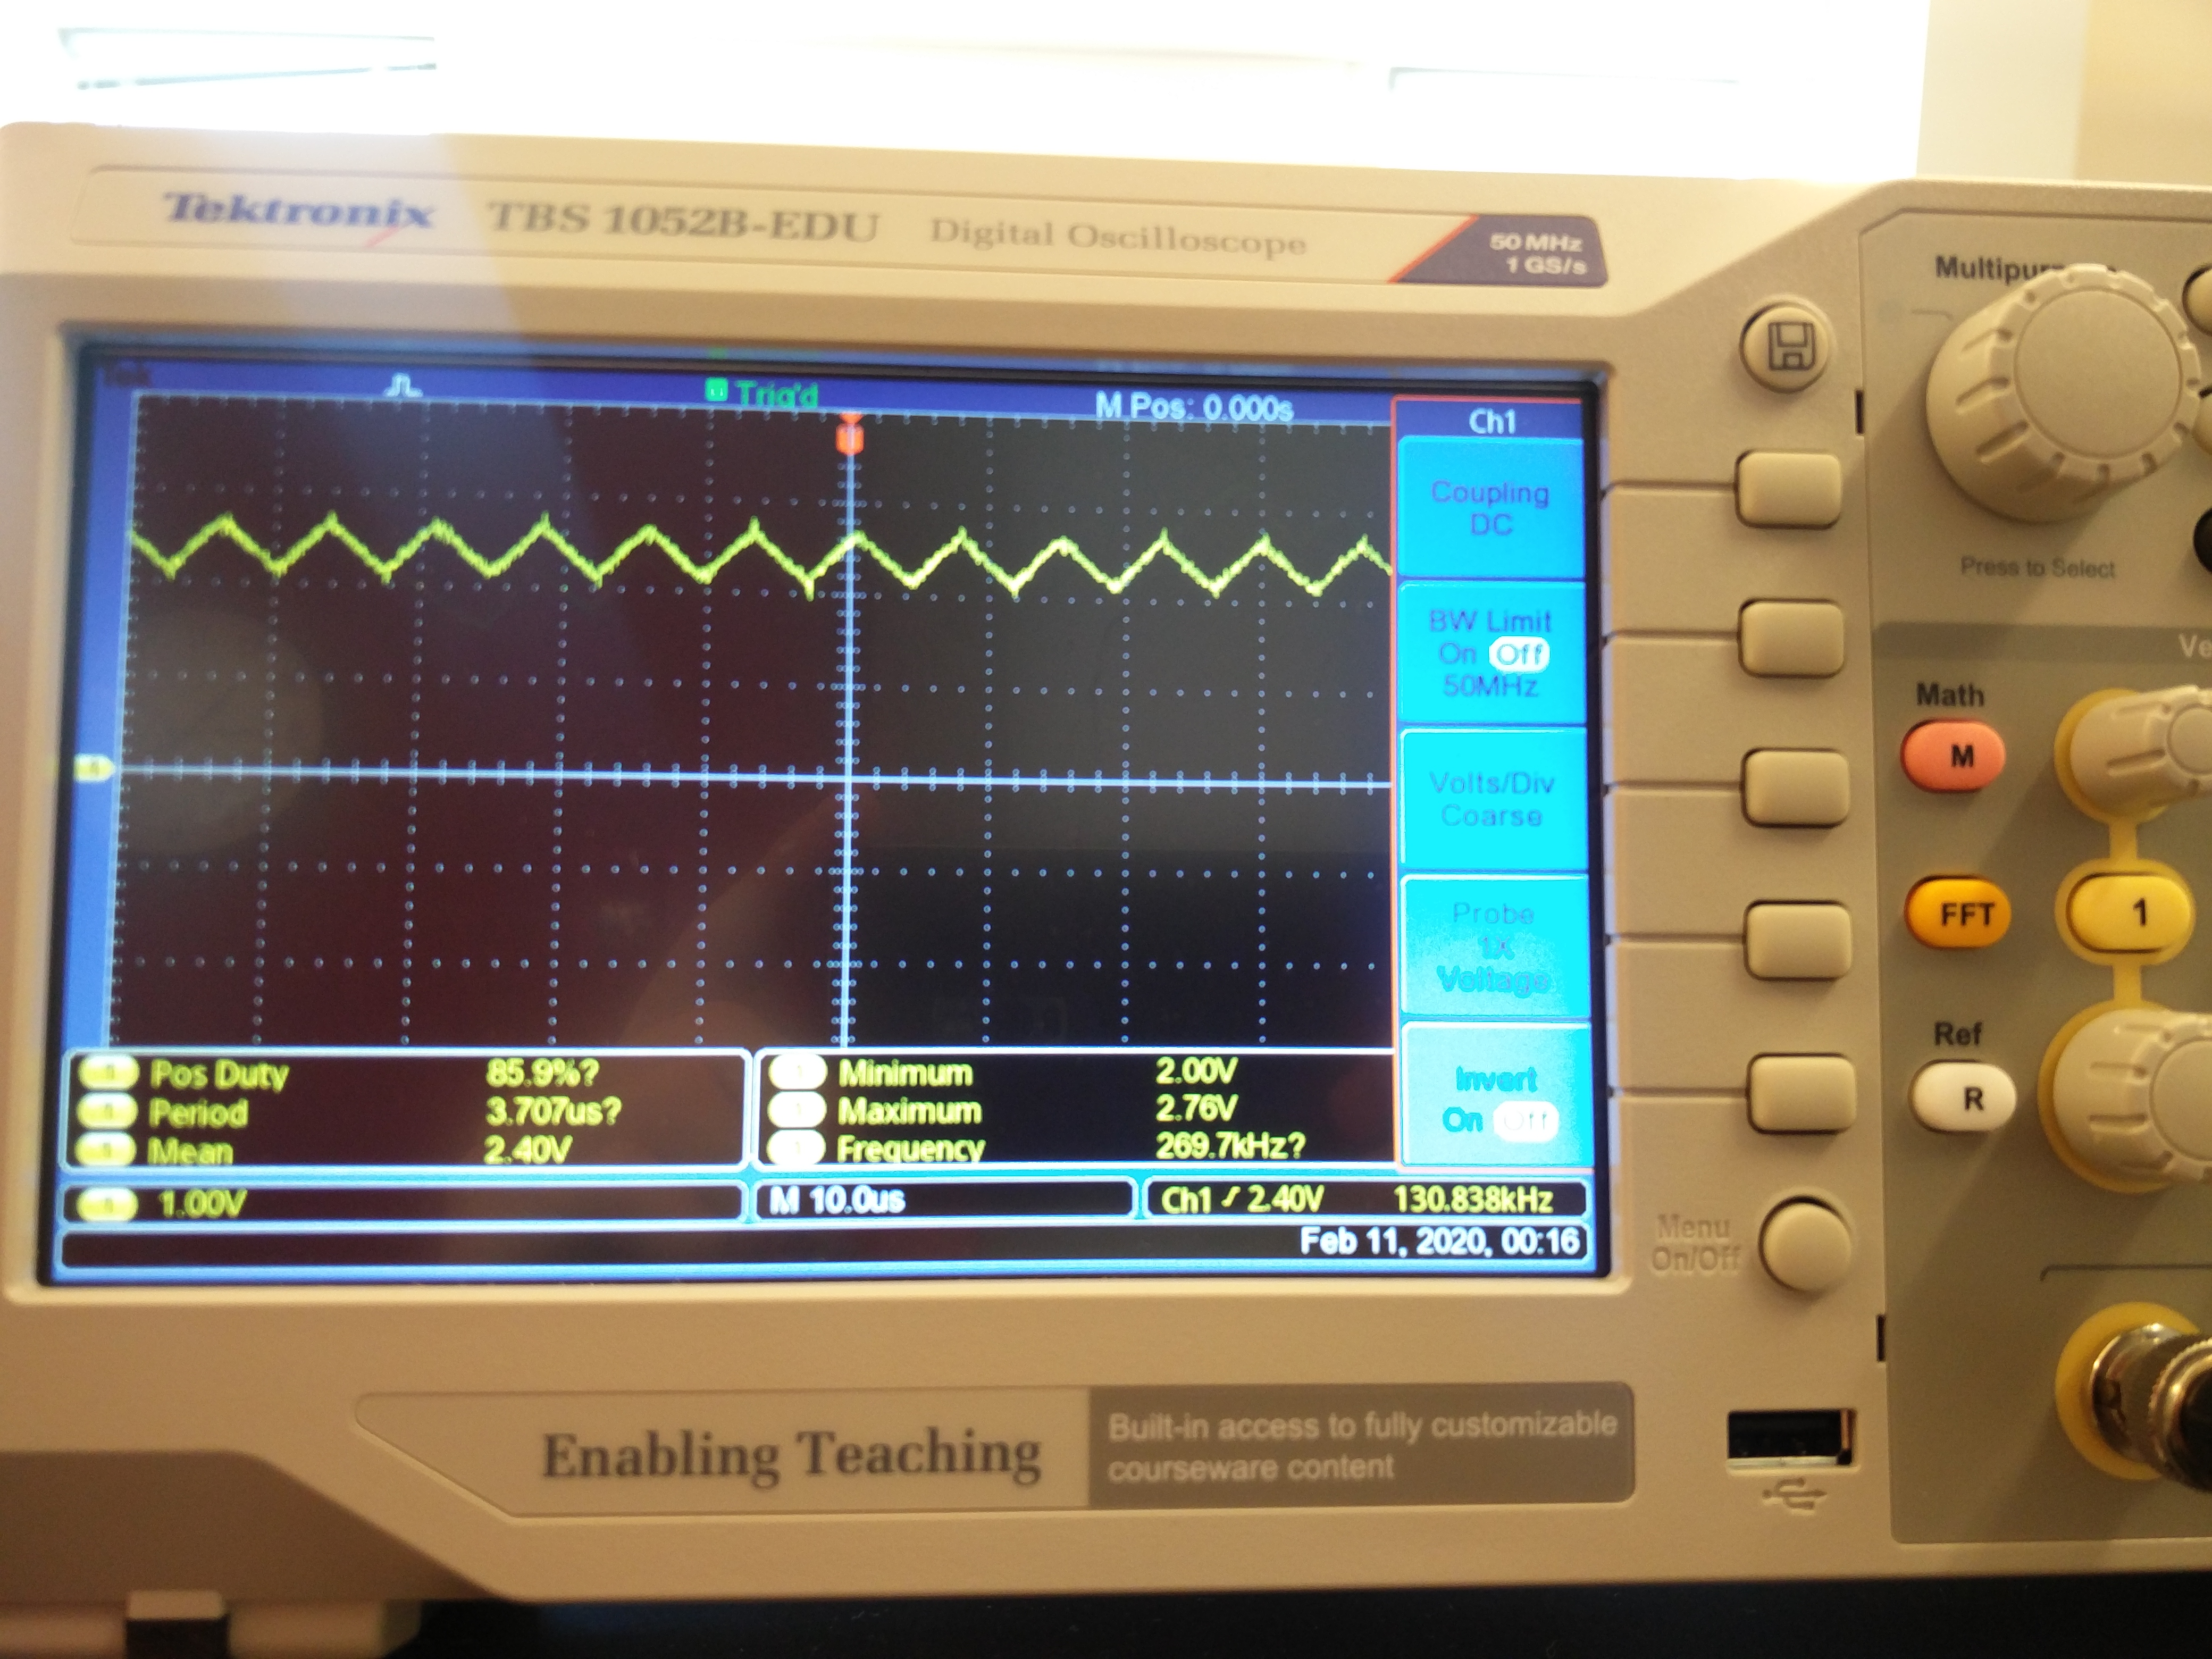
\includegraphics[width=3.5in]{sawTooth.jpg}
	\caption{Simple Sawtooth Wave}
	\label{fig1}
\end{figure}

\section{Sine Wave}
A sine wave is a little more complicated though. Fortunately this one is entirely software tweaks from the sawtooth. So instead of a linear increase and decrease of the pwm duty, we need it to follow that of a sine wave. The Arduino library has a built in sine function that we can use, but there's a problem that we need to address first. The functions input ranges from -2$\pi$ to 2$\pi$. This is all well and good. But the output ranges from -1 to 1, but we need the output to form our duty cycle, in this case from 0 to 1. We can start by adding 1 to the function output. This will bring the output to [0, 2], and then we can easily divide it by 2 to achieve our [0, 1]. This function can be see below.

\begin{equation}
	\frac{sin([-2\pi, 2\pi])+1}{2} = [0, 1]
\end{equation}

This function output can then be shaped to form whatever type of sine wave you need. An example of this sine wave can be seen below.

\begin{figure}[ht]
	\centering
	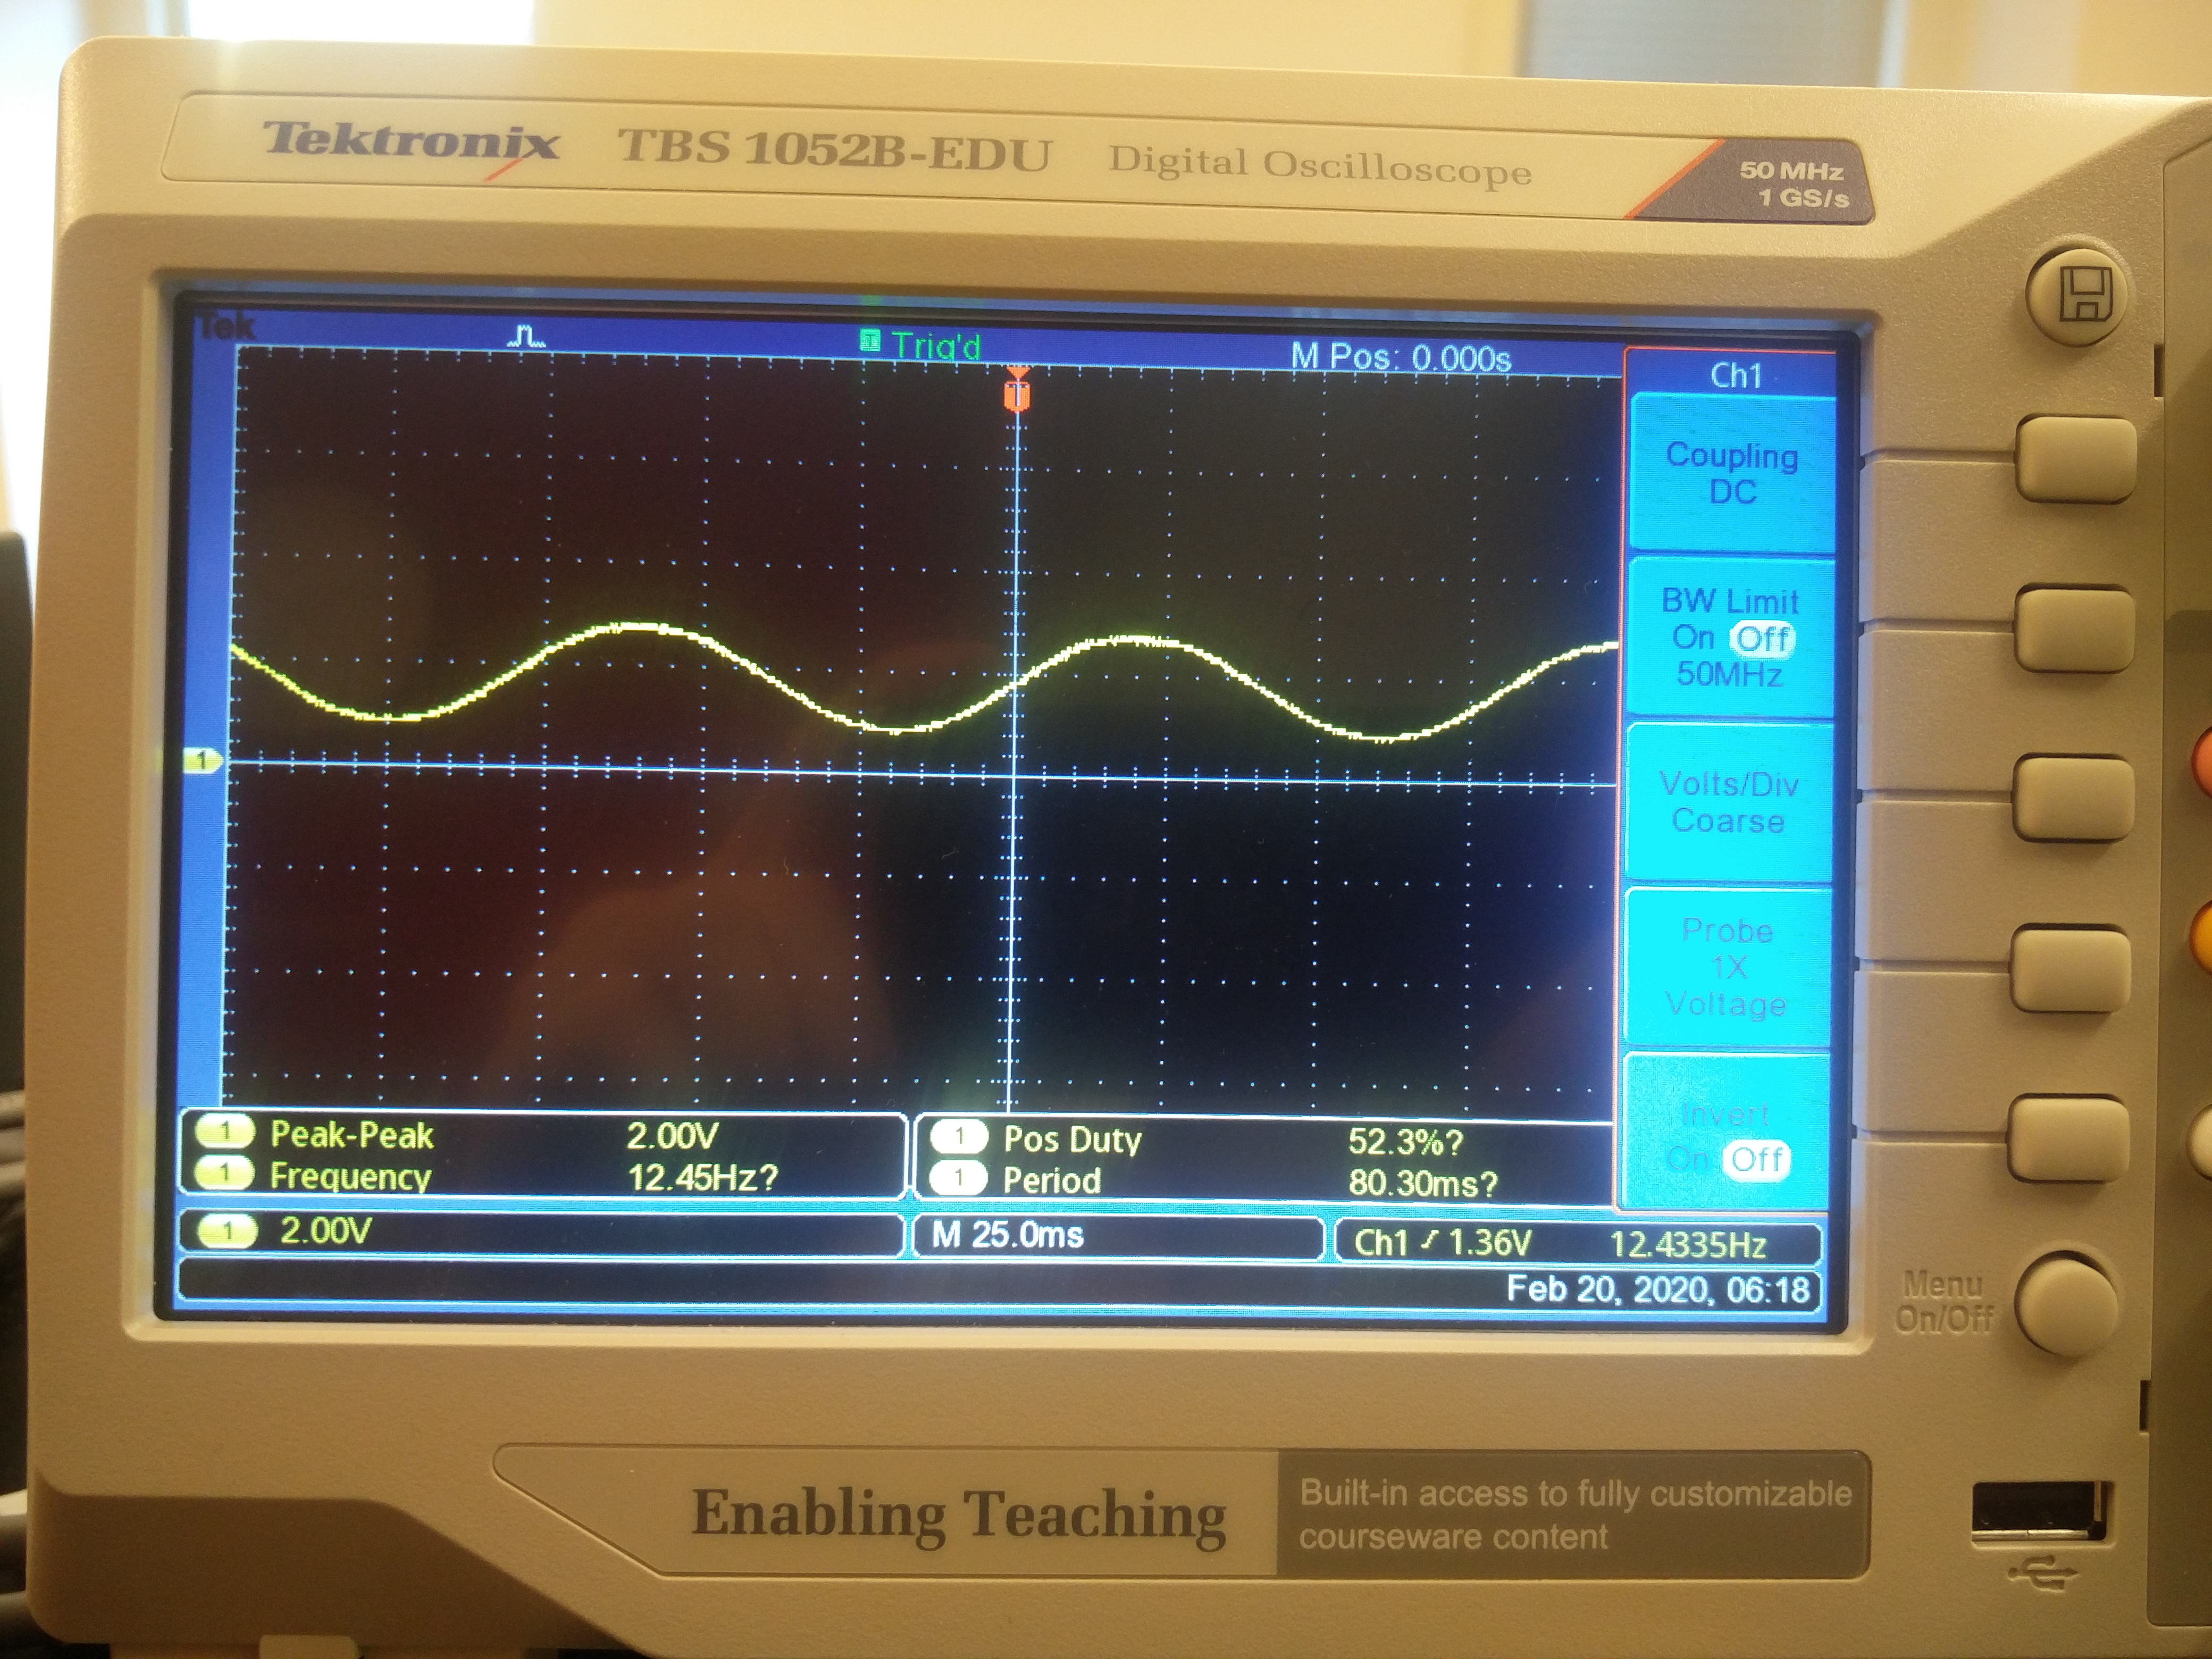
\includegraphics[width=3.5in]{sineWave.jpg}
	\caption{Simple Sine Wave}
	\label{fig1}
\end{figure}

%\begin{thebibliography}{99}
% The numeral (here 99) in curly braces is nominally the number of entries in
% the bibliography. It's supposed to affect the amount of space around the
% numerical labels, so only the number of digits should matter--and even that
% seems to make no discernible difference.
%Not Requested
%\end{thebibliography}

\end{document}
